\documentclass[a4paper,twocolumn,5p]{elsarticle}

\usepackage[draft]{hyperref}
\usepackage{url}
\usepackage{booktabs}
\usepackage{graphicx}
\usepackage{xspace}
\usepackage{booktabs}
\usepackage[draft,inline,nomargin]{fixme}
\usepackage{makecell}
\usepackage[columnwise]{lineno}
\usepackage{natbib}
\DeclareRobustCommand{\citeext}[1]{\citeauthor{#1}~\cite{#1}}

\journal{Environmental Pollution}

%% `Elsevier LaTeX' style
\bibliographystyle{elsarticle-num}
%%%%%%%%%%%%%%%%%%%%%%%

\begin{document}
\pagewiselinenumbers

% Macro para escribir NO$_2$
\newcommand{\no}{NO\textsubscript{2}\xspace}

\begin{frontmatter}

  \title{Forecasting the full distribution of \no concentrations to
    anticipate pollution peaks
%    extreme pollution episodes% \\
    % Extreme pollution episodes: forecasting the full
    % distribution of \no concentrations
  }

\author{Sebasti\'an P\'erez Vasseur} 
\address{Artificial Intelligence Department\\Universidad Nacional de
  Educaci\'on a Distancia --- UNED\\c/ Juan del Rosal, 16, Madrid, Spain}

\author{Jos\'e L. Aznarte\fnref{myfootnote}}
\address{Artificial Intelligence Department\\Universidad Nacional de
  Educaci\'on a Distancia --- UNED\\c/ Juan del Rosal, 16, Madrid, Spain}
\ead{jlaznarte@dia.uned.es}


\begin{abstract}
  % Air quality is an increasingly alarming issue in cities around the
  % world and thus there is an urgent need to reliably forecast high
  % concentration episodes of certain pollutants in the air. In this
  % sense, \no is one of the most worrisome pollutants, as it has been
  % proven its direct implication in a variety of serious health
  % affections. In some cities, high concentration episodes for \no are
  % dealt with by authorities through traffic restriction measures,
  % amongst others, which are activated when air quality deteriorates
  % beyond certain thresholds.

  High concentrations of pollutants in the atmosphere, whose direct
  implication in a variety of serious health affections is widely
  accepted, represent an alarming issue around the world. In some
  cities, high concentration episodes for \no are dealt with by
  authorities through traffic restrictions which are activated when
  air quality deteriorates beyond certain thresholds. Forecasting
  pollutant concentrations becomes thus a necessity both for decision
  makers and the general public.

  Probabilistic forecasting is an approach that % (as opposed to deterministic or point
  % forecasting, which is designed to predict a single expected value),
  allows for the prediction of the expected distribution function for
  any magnitude. In the case of \no, this is a key feature which
  allows for the calculation of the future probabilities of exceeding
  the protective thresholds as well as to derive cost-effectiveness
  analysis or to %. Probabilistic forecasting is also specially useful to
  detect pollution peaks, which usually are rare events.

  In this study, we have % extended previous research on forecasting
  % future \no concentrations with the implementation of
  implemented four different probabilistic predictive models: a
  probabilistic version of $k$-nearest neighbors, quantile random
  forests, linear quantile regression and quantile gradient boosted
  trees.  We have used those models to predict \no concentrations in a
  precise urban location
  % a wide set of forecasting horizons (up
  % to 60 hours)
  , and we have studied the quality of the forecasts.  We have also
  improved some of those models by applying a novel nested scheme to
  the output of a linear model. In our experiments, quantile gradient
  boosted trees is the best performing model as it provides the best
  results for both the expected value and the forecast full
  distribution. Furthermore, we show how this approach can be used to
  detect pollution peaks with almost no false positives.
\end{abstract}

\begin{keyword}
probabilistic forecasting \sep air quality \sep quantile regression
\sep nitrogen dioxide \sep Madrid
\end{keyword}

\end{frontmatter}

%\linenumbers

\section{Introduction }
\label{sec:intro}

Pollution has become a worrying issue in cities due to its adverse
effects on health and the increase in pollutant concentrations, mainly
due to human activity (traffic, heating systems\ldots). In order to
take preventive steps to maintain air quality, forecasting the
evolution of pollution levels becomes a useful tool for decision
makers: detecting pollution peaks beforehand could give cities enough
time to take and communicate effective measures.

Multiple research papers have focused on this issue and have dealt
with the prediction of air quality. Bai et al. \cite{bai_air_2018}
describes the state of the art in this exercise and collects a range
of diverse solutions applied to this problem.

However, the prediction of the expected value of pollution
concentrations through point-forecasting does not provide enough
information about the likelihood of the pollutant levels reaching a
certain threshold. Indeed, we have an estimate but we usually do not
have a description of the confidence of the model nor the uncertainty
in the predictions. Therefore, it is difficult to estimate the
probability of the pollutant reaching above a certain threshold.

The reason this probability estimation is so important is because the
measures taken by cities to limit pollution (for example, limiting
traffic) impact the daily routines of citizens and prove themselves to
be quite unpopular.  Therefore, local governments need to have an
estimation of the confidence in the prediction to safely engage in
those preventive measures.

% Also the use of a classifier (above or below threshold) can not 
% be used. First, we would need a classifier per threshold, but 
% more importantly, pollution peak is an extremely rare event and 
% classifiers would have to be trained with high imbalanced datasets.

As noted by Hothorn \emph{et al.} \cite{hothorn_conditional_2014}, the
real objective in a regression analysis is to find the conditional
distribution of the target variable: in our case, the full
distribution of the concentration of the pollutants. Indeed, this full
distribution gives an idea of the uncertainty of our predictions and
can be useful to forecast the probability of the signal being above a
certain threshold. For example, in the city of Madrid, \no
concentrations in the air are considered to be harmful from 180
$\mu g / m^3$.

Previous research on the same dataset has already shown the usefulness
of probabilistic forecasting for \no levels \cite{proba_aznarte},
establishing the advantages of the approach and focusing on 1
hour-ahead predictions with a single model (quantile random
forests). We hereby extend that work by implementing other models
(quantile linear regression, quantile gradient boosted trees % , quantile
% random forests
and quantile $k$-nearest neighbors) and using them for
a wide set of forecasting horizons (up to 60 hours). Inspiration is
drawn on some of the best approaches from the GEFCom Competition
\cite{mangalova_k-nearest_2016,hong_probabilistic_2016}.

Furthermore, improving over these approaches, we also present a novel
method to apply statistical inference to the output of the
models. This method aknowledges the fact that the results show linear
dependences between the predictors and the target, which slightly
benefits linear models over nonlinear ones. By combining a linear
model with nonlinear probabilistic modelling of its residuals we
obtain optimized versions of the standard models.
% This way, we are
% converting our forecasting method into a semi-parametric model.

Finally, in order to showcase one of the applications of probabilistic
forecasts, we tackle the prediction of \no peaks for the different
horizons, and compare the performance of the proposed models on this
task. 

\section{Probabilistic forecasting with quantile regression}
\label{sec:probForec}

The prediction from most regression models is a point estimate of the
conditional mean of a dependent variable, or response, given a set of
independent variables or predictors. However, the conditional mean
does not provide a complete summary of the distribution, so in order
to estimate the associated uncertainty, quantiles are in order. The
0.5 quantile (i.e., the median) can serve as a measure of the center,
and the 0.9 quantile marks the value of the response below which
reside the 90\% of the predicted points. Recent advances in computing
have inducted the development of regression models for predicting
given quantiles of the conditional distribution. The technique is
called quantile regression (QR) and was first proposed by Koenker in
1978 \cite{koenker_quantile_2001} based on the intuitions of the
astronomer and polymath Rudjer Boscovich in the 18th
century. Elaborating from the same concept of estimating conditional
quantiles from different perspectives, several statistical and CI
models that implement this technique have been developed: from the
original linear proposal to multiple or additive regression, neural
networks, support vector machines, random forests etc.

Quantile regression has gained an increasing attention from very
different scientific disciplines \cite{yu_quantile_2003}, including
financial and economic applications \cite{ben_rejeb_financial_2016},
medical applications \cite{jang_quantile_2018}, wind power forecasting
\cite{wan_direct_2017}, electric load forecasting
\cite{lebotsa_short_2018}, environmental modelling
\cite{cade_gentle_2003} and meteorological modelling
\cite{baur_modelling_2004} (these references are just examples and the
list is not exhaustive). To our knowledge, despite its success in
other areas, quantile regression has not been applied in the framework
of air quality , with the exception of
\cite{martinezsilva_forecasting_2016}.

Thus, as we can estimate an arbitrary quantile and forecast its
values, we can also estimate the full conditional distribution, which
will entail us to the results presented in Section \ref{sec:results}.

Among the growing array of methods that allow to estimate and forecast
data-driven conditional quantiles, in this study we have chosen to
compare linear regression, $k$-nearest neighbors, random forests and
gradient boosted trees. We took the point-estimate version of those
models and converted them to their quantile or probabilistic
counterparts. We can therefore compare each model not only on the
accuracy of their point estimation but on the confidence of each
model.

We will compare the different algorithms through the RMSE, MAE and
bias for the quantile 50 and the CRPS metric for the forecast
distribution.  As described by Gneiting et
al. \cite{gneiting_probabilistic_2014}, CRPS is a measure of the
squared difference between the forecast cumulative distribution
function (CDF) and the empirical CDF of the observation.

\section{Data description and experimental design}

\subsection{Nitrogen dioxide}
\label{sec:no2}

\begin{figure}
  \centering
  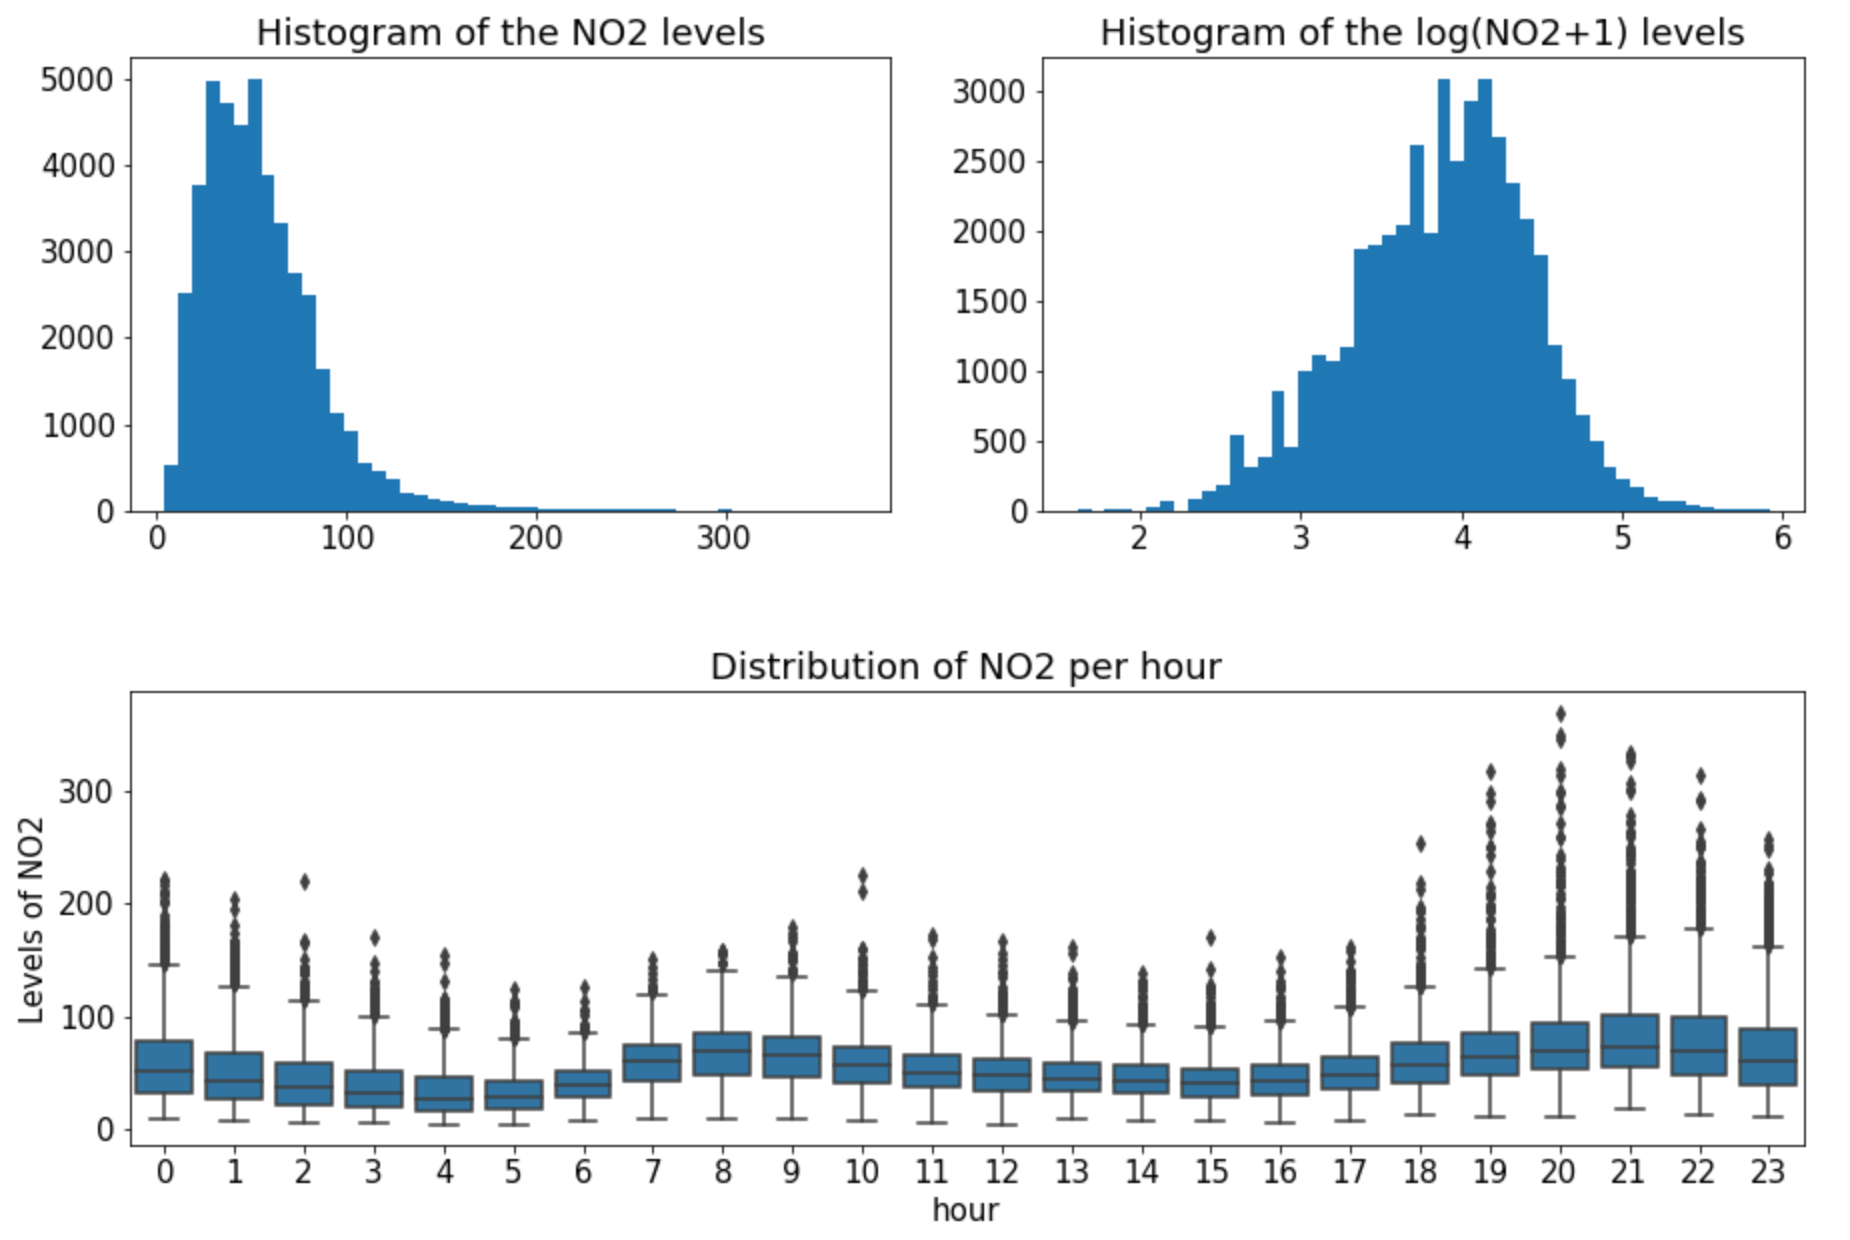
\includegraphics[width=0.5\textwidth]{histo_variance}
  \caption{\label{figure:histo_variance}Distribution of logarithmic
    NO\textsubscript{2} and Distribution of NO\textsubscript{2}
    per hour.}
\end{figure}

The city of Madrid has an air quality monitoring system composed by 24
stations which capture hourly data for \no.  For this study, we have
selected one of the stations with higher average leves: Escuelas
Aguirre station (code 28079008).

As we can see in \ref{figure:histo_variance}, the shape of the histogram
approaches the one from a lognormal distribution and therefore we
transformed to the logarithm of the values. This has 2 positive
effects: it reduces the tail of the distribution which will enable
better quantile estimation and it reduces the skewness of the
distribution which helps with linear models like the linear quantile
regression.

The time series for this station consists of hourly measured values of
the concentrations of \no from 01/01/2013 to
30/11/2017. These values exhibit a clear intraday pattern, in which
the higher values are located in two peaks around the morning and
evening (with highest average value around 19h) while the nightly
hours (from 00h to 05h) have lower average concentrations.  Not only
are the values higher at those hours, but also the variance is, as we
can see in figure \ref{figure:histo_variance}.
 
In order to analyze the seasonality of the signal, we extract the 5
main factors from the Fourier transform. Those correspond to the main
repetitive patterns found on the series, and can be seen clearly from
the first 3000 components. The series shows certain seasonality for
12-hour, 24-hour, one week (168-hour) and one year.  Therefore, we will
create, and use as inputs for the models, the output of periodic
functions (cosine and sine) whose frequency is equal to the ones
stated above. This will enable the machine learning models to learn
the seasonality of our time series.

As is common when forecasting with machine learning models, we exploit
the inertia of the modelled series by adding lagged variables to the
inputs. Of course, in doing so, we are limited by the horizon of the
prediction and by the 'curse of dimensionality', which implies keeping
a limited number of features as input. In our case, the inertia of the
series will be modeled by lagged values from the inmediate past (hours
before) and, based on the seasonal analysis: 1-5 hours before and
every 11-13 hours up to 9 days before.

\subsection{Ozone}

\begin{figure}
  \centering
  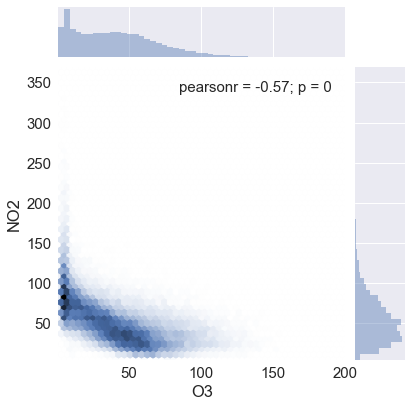
\includegraphics[width=0.4\textwidth]{no2vso3}
  \label{figure:no2vso3}
  \caption{Dispersion of levels of $O_3$ vs. levels of $NO_2$.}
\end{figure}

The same station that records Nitrogen dioxide also records the levels
of ozone (O\textsubscript{3}). It is known that ozone and Nitrogen
dioxide are related by chemical reactions occurring in the atmosphere
in the presence of sunlight, especially of the UV spectrum.  As we can
see in figure \ref{figure:no2vso3}, there seems to be a correlation
between NO\textsubscript{2} levels and O\textsubscript{3}. Thus, we
will also add lagged values of O\textsubscript{3} as inputs to our
models.

\subsection{ECMWF numerical pollution prediction}
\label{sec:ecmwf-numer-poll}

The European Centre for Medium-Range Weather Forecasts (ECMWF)
implements the Copernicus Atmosphere Monitoring Service.  This service
delivers a daily production of near-real-time European air quality
analyses and forecasts with a multi-model ensemble system. Although
these forecasts are a very good starting point, 
the resolution of the model is 10km
and hence it is not expected to be capable of modelling the local
urban effects of the NO\textsubscript{2} series under study.

\subsection{Calendar Variables}
\label{sec:cal_data}

As NO\textsubscript{2} levels are clearly be linked to human activity,
we will also flag the hours belonging to a specific type of day. Days
could be classified as bank holidays, heavy traffic days (for example,
return from holidays), school holidays\ldots We will also use as
inputs to the models past values of this variables ( 1,2 and 7 days
before).

\subsection{Experimental Design}
\label{sec:experimental-design}

\begin{figure}
  \centering
  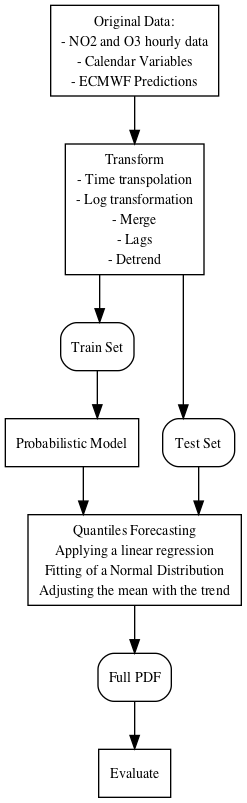
\includegraphics[width=0.15\textwidth]{diagrams/flow}
  \caption{\label{figure:dataflow}Data flow of the
    experiments.}
\end{figure}

As a summary, we use the following predictors: \no
measures lagged 1-5H and every 11-13H up to 9 days before,
O\textsubscript{3} levels lagged every 24H up to 4 days before, 
calendar variables lagged 1,2 and 7 days before,
 ECMWF predictions and seasonal features extracted
from the Fourier analysis. This amounts to a total of 102 independent
variables. 

When performing the experiments, first we aligned and gathered all the
hourly time series: \no, O\textsubscript{3}, ECMWF and
calendar variables.  Then we transformed the signal levels and then we
added the lagged values and a seasonal time series with the main
periods of the NO\textsubscript{2} time series.

Once all this process is finalized, we train the following
probabilistic models: quantile random forests (QRF), $k$-nearest
neighbors (QKNN), quantile linear regression (QLR) and quantile
gradient boosting (QGB).  Figure \ref{figure:dataflow} shows the data
flow in the experimental design. All the hyperparameters of the models
have been estimated through grid search on a validation set.  
In Section \ref{sec:models}
we provide more information on each of the models.

Concerning cross-validation, there are several accepted methods to
separate the train and test set which produce correct estimations of
the error \cite{bergmeir_note_2018}. We use the out-of-sample
approach: train the models with data prior to 2017 and test our models
with data from 2017. We will always test with predictions done at
10:00, as this is the time the forecast is done in the operational
setting, as the data is first available at that time.

We want to forecast the full distribution of \no
levels for the next 60 hours and therefore we will train and evaluate
the models for each hour (60 horizons).

After forecasting the quantiles, we will fit them to a normal
distribution. Fitting a normal distribution to the predicted quantiles
and then generating the percentiles for that fitted distribution has
several advantages. It enables the calculation of more percentiles
from a small number of them.  It also helps estimating the upper tail
of the distribution, in spite of the low probability for those values.

We will evaluate the predicted 50 percentile through standard
evaluation metrics (RMSE, MAE and bias), and the predicted
distribution through the continuous ranked probability score (CRPS).

We will perform this evaluation for
each of the models and each of the horizons.

\subsection{Probabilistic Models}
\label{sec:models}

As stated above, we will compare four different probabilistic models,
which are briefly described below for reference. We will provide 
alongside the models the abreviation we will use for each of them 
throughout this article. Also we are adapting point-estimation 
algorithms to their probabilistic counterparts. This allows 
us to see the uncertainty these models have. Indeed, metrics like 
RMSE and Bias are linked to the confidence of the models for 
point estimation but the predicted CDF is much better at describing 
it. This also increases the interpretability of those models.
Therefore 
the implementations we described can have applications beyond 
this forecast exercise.

\subsubsection{Quantile linear regression (QLR)}

As shown in \cite{koenker_quantile_2001}, we can apply linear
regression with a modified cost function in order to predict the
quantiles of the dependent variable.  Given a set of vectors
$(x_i, y_i)$, in the usual point forecasting approach we are usually
interested in the prediction $\hat y(x) = \alpha_0 + \alpha_1 x$ which
minimizes the mean squared error,
\begin{equation}
  \label{eq:1}
  E = \frac{1}{n} \sum^n_i \epsilon_i =
  \frac{1}{n} \sum^n_i [ y_i - (\alpha_0 + \alpha_1 x) ]^2.
\end{equation}
This prediction is the conditional sample mean of $y$ given $x$, that
is, $\hat y(x) = \hat\alpha_0 + \hat\alpha_1 x$, or the location of
the conditional distribution. But we could be interested in estimating
the conditional median (i.e., the 0.5 quantile) instead of the mean,
in which case we should find the prediction $\hat y(x)$ which
minimizes the mean absolute error,
\begin{equation}
  \label{eq:2}
  E = \frac{1}{n} \sum^n_i \epsilon_i =
  \frac{1}{n} \sum^n_i | y_i - (\alpha_0 + \alpha_1 x) |.
\end{equation}

The fact is that, apart from the 0.5 quantile, it is possible to
estimate any other given quantile $\tau$. In that case, instead of
(\ref{eq:2}), we could minimize
\begin{equation}
  \label{eq:3}
  E= \frac{1}{n} \sum^n_i f( y_i - (\alpha_0 + \alpha_1 x))
\end{equation}
where
\begin{equation}
  \label{eq:4}
  f(y-q) = \left\{ 
    \begin{array}{l l}
      \tau (y-q) & \quad \mbox{if $y \ge q$}\\
      (1-\tau) (q-y) & \quad \mbox{if $y < q$}\\
    \end{array} \right.,
\end{equation}
with $\tau \in (0,1)$. Equation (\ref{eq:3}) represents the median
when $\tau=0.5$ and the $\tau$-th quantile in any other case.

We will train 5 linear regression models to predict 5 percentiles of
the signal. As percentiles are calculated separately, we have the risk
of quantile crossing.  We will reorder the quantiles as explained in
\cite{cross} to solve this problem.

\subsubsection{Quantile $k$-nearest neighbors (QKNN)}

We will use the probabilistic $k$-nearest neighbors algorithm as
described in \cite{quantileknnmangalova}.  This algorithm is based on
the standard $k$ nearest neighbor, where instead of calculating the
mean of the targets of the $k$ nearest points to the input, it builds
a distribution from the target of those neighbors.

\subsubsection{Quantile random forests (QRF)}

Quantile random forests create probabilistic predictions out of the
original observations. They work like the usual random forest, except
that, in each tree, leafs do not contain a single value as a
prediction but the target observations from the training set belonging
to that
leaf.

Then predictions are calculated by selecting the leafs in each tree
corresponding to the input features and combining the weighted
histograms in each tree out of the target observations in those leafs.
For more information refer to \cite{quantregforests}.

\subsubsection{Quantile Gradient Boosted Trees (QGB)}

Tree boosting \cite{friedman_greedy_2001} is a recent and successful
machine learning technique that consist on growing trees based on the
compromise of a cost function and a regularization function. This cost
function is usually used to forecast the mean of the signal. We will
modify the cost function (im a similar way as in the quantile linear
regression) to predict the quantiles of the target. Also, we will use 
the lightgbm implementation \cite{ke_lightgbm:_2017} which provides 
lower training times and higher accuracy.

We will train 5 gradient boosted trees models to predict 5 percentiles
of the \no signal and we will solve quantile 
crossing with the technique
explained in \cite{cross}.

\section{Results and discussion}
\label{sec:results}

\begin{figure}[tbp]
  \centering
  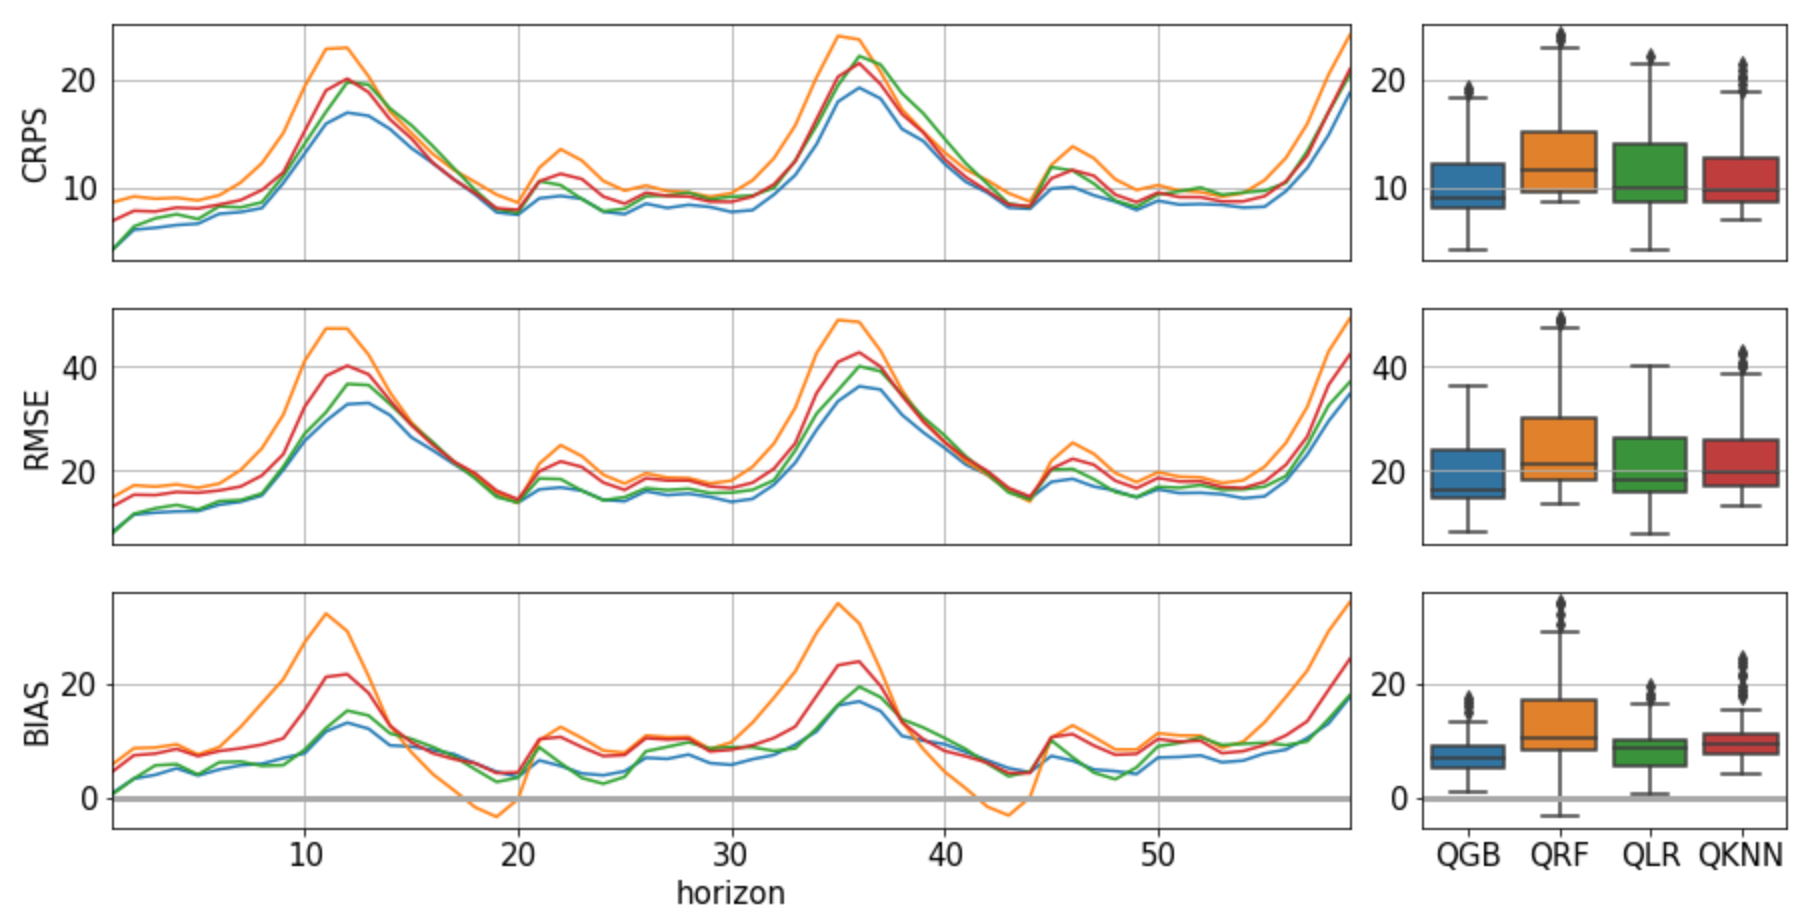
\includegraphics[width=0.48\textwidth]{error_graph}
  \caption{\label{figure:errorGraph}
    Continuous ranked probability score, root mean squared
    error and bias of the different models with respect to the
    forecasting horizon and in average.
  }
\end{figure}

\begin{table}[tbp]
  \centering
  \caption{\label{tab:determ}CRPS Error for the proposed models at different
    horizons.}
  \begin{tabular}{lrrrr}
    \toprule
    & \multicolumn{4}{c}{Model} \\ \cmidrule{2-5} 
    h &    QGB &  QKNN &   QLR &   QRF \\
    \midrule
    1     &  4.21 &   4.14 &  4.21 &  4.30 \\
12    & 16.96 &  18.04 & 19.79 & 17.93 \\
13    & 16.66 &  17.32 & 19.56 & 17.58 \\
14    & 15.43 &  15.57 & 17.35 & 15.96 \\
20    &  7.46 &   7.48 &  7.64 &  7.50 \\
37    & 18.26 &  18.75 & 21.42 & 19.02 \\
45    &  9.87 &  10.39 & 11.88 & 11.05 \\
55    &  8.20 &   8.15 &  9.69 &  8.67 \\

    \midrule
    average & 10.39 &  10.57 & 11.59 & 10.73 \\
    \bottomrule
  \end{tabular}
\end{table}

\begin{figure}
  \centering
  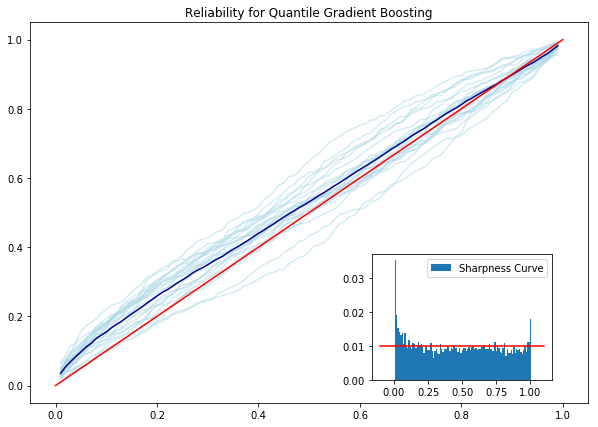
\includegraphics[width=0.45\textwidth]{reliability_sharpness}
  \caption{\label{figure:rel_sharp}Average reliability and sharpness
    of the different models across all horizons. The dim blue lines
    correspond to the different horizons. }
\end{figure}

Figure \ref{figure:errorGraph} shows the different metrics for each
model across all the horizons. First, we clearly see how 
quantile gradient
boosted trees outperform the other models and displays better scores
for all metrics.

Secondly, we can observe how quantile random forests and 
quantile $k$-nearest
neighbors underperform compared to the other models, showing a bias
which is clearly higher compared to the others.  The main reason for
this is the high linear dependence of the data. This also explains
then the good results of the linear model (QLR).  However, the linear
model underperforms when compared to gradient boosted trees, as it is
not able to learn the non-linear relationship between the predictors
and the target.

As stated earlier, the \no levels follow a lognormal
distribution and it seems that it is better modelled with a
multiplicative model (different causes multiply the level of
pollution), therefore the logarithm of the \no levels
are better forecast with an additive model. 
This is the reason why
quantile gradient boosted trees outperform 
the other models: it can naturally
add the nonlinear effects.

Table \ref{tab:determ} displays the CRPS of the different models at
some selected prediction horizons. The table shows again the good
performance of the quantile 
gradient boosted trees model for CRPS.

For probabilistic models, CRPS is a good summary of the performance of
the models. Notwithstanding, the reliability and sharpness graphs are
known to be useful at estimating how the observed values are
positioned in the distributions.  Figure \ref{figure:rel_sharp}
features the reliability and sharpness of the different models.

The sharpness curve shows that quantile random forests 
and quantile $k$-nearest
neighbors tend to underestimate the levels of
\no. This is clear in the sharpness curve for the
upper percentiles. The observed values of those percentiles are
usually noticeably higher than the forecast values. This means that,
too many times, the observed values are in the upper percentiles of
the distribution. This is also a consequence of the bias of both
models.

Gradient boosted trees and quantile linear regression forecast
distributions seem more balanced but display high values at both sides
of the sharpness curve.  If we consider the distribution to be a
gaussian distribution, this means the forecast distributions tend to
have a too small standard deviation and are too narrow. Therefore, the
forecast probability of some levels of \no is too
small compared to the observed one.

\subsection{Probabilistic forecast of linear regression residuals}

\begin{figure}[tbp]
  \centering
  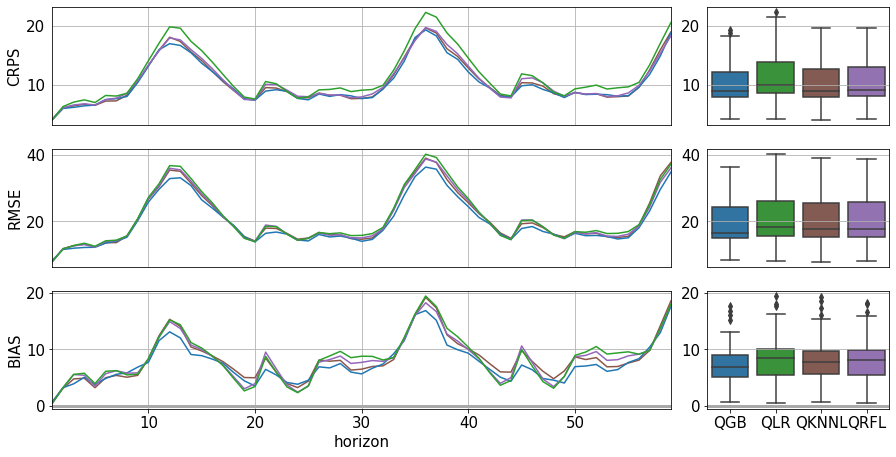
\includegraphics[width=0.48\textwidth]{errorGraph_rfl_knnl}
  \caption{Continuous ranked probability score, root mean squared
    error and bias of the different models with respect to the
    forecasting horizon and in average.}
  \label{figure:errorGraph_rfl}
\end{figure}

As stated before, the results show linear dependences between the
input predictors and the target. This fact explains why we obtained
poorer results for quantile $k$-nearest neighbors and quantile random
forests than for the linear quantile model. However, we can improve
the results by combining both approaches.

We decided to train a linear regressor which predicts the
\no values and then use the quantile random forest and quantile
$k$-nearest neighbor to predict the full distribution of the residuals
of that linear regression. We abbreviate both models respectively with
QRFL and QKNNL.

We obtained much better results and we brought a real improvement to
the predictions. Figure \ref{figure:errorGraph_rfl} shows the updated
metrics with the new models, where we can see the comparison with the
original gradient boosted tree (QGB) and quantile linear regression
(QLR) models. Due to the additive nature of the gradient boosted trees
method, this technique does not bring improvement to this type of
model.

Also, we still see the combined models underperforming against
quantile gradient boosted trees, which keeps the first position in all
the error measures. The additive nature of QGB is behind these
results. 

\subsection{Comparison of the prediction on selected days}

\begin{figure*}
  \centering
  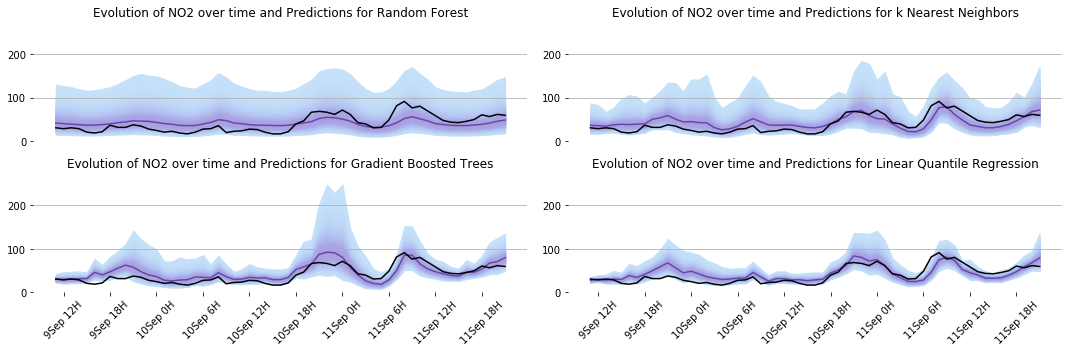
\includegraphics[width=0.75\textwidth]{evoday1}
  \caption{Forecasts of the four models on September, 9th
    2017.}
  \label{figure:evoday1} 
\end{figure*}

\begin{figure*}
  \centering
  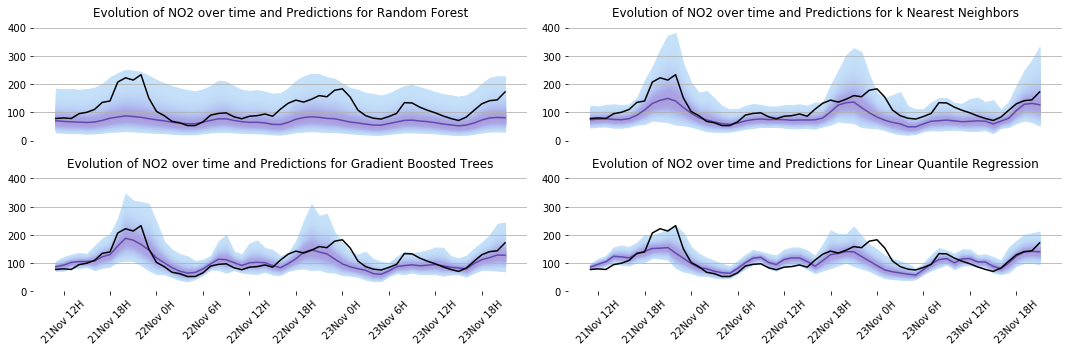
\includegraphics[width=0.75\textwidth]{evoday2}
  \caption{Forecasts of the four models on November, 21st 2017.}
  \label{figure:evoday2} 
\end{figure*}

As an example of the capabilities of the four models, Figure
\ref{figure:evoday1} and \ref{figure:evoday2} compare their forecasts
in 2 different days: one day with low \no levels and
another with levels above the health threshold of 180 $\mu gm^{-3}$.
As stated earlier, the predictions were done at 10:00 AM and we
forecast the distribution of the concentration for the next 60 hours.

We see more clearly in those examples how the quantile random forests 
tend to
underestimate the target and misses to build a meaningful distribution
as it is not fitting well the data. On the other hand, 
quantile $k$-nearest
neighbors does a better job but the upper percentiles of the
distribution are too high.  Finally we ca visualize how quantile linear 
regression and quantile gradient boosted trees fit better the 
data with quantile gradient boosted trees outperforming
 on high values.


\subsection{Forecasting \no concentration peaks}

One of the applications of probabilistic forecasts is the estimation
of the probability of the signal being above a certain threshold. In
the case of \no forecasting, this is especially useful when normative
limits are established by authorities.

We evaluated the proposed models to check how good are they to detect
those peaks.  In Madrid, municipal regulations fix a threshold of 180
$\mu gm^{-3}$ to activate the first level of restrictive measures on
traffic. Thus, we consider that a \no peak is forecast when the
probability of reaching above this limit is higher than 50\%.  It is
important to note that this normative threshold lies around the 99.7
quantile of the \no distribution, and thus it is safe to consider
peaks as rare events.
This fact of course implies that the possibility of using a classifier
to predict peaks, with classes above or below the threshold, is not
straightforward. Firstly, we would need a classifier per threshold,
but more importantly, it would suffer from the fact that the training
dataset would be highly imbalanced.

As noted before, there is usually a high cost on performing preventive
measures against pollution. This has some consequences for the
evaluation of our models. We must minimize the number of false
positives and false negatives and thus secondary metrics like the ROC
curve are not directly applicable as in this case, depending on the
take of the decision makers, the cost of a false positive might be
much higher than the cost of a false negative. Table
\ref{table:classif_hig} shows the true positives and false positives
of each model. We see again the superior results of quantile gradient
boosted trees against the other models.

\begin{table}[tbp]
  \centering
  \caption{\label{table:classif_hig}
    Detection of \no peaks (above 180 $\mu gm^{-3}$) with the proposed
    models for a selection of horizons. TP and FP stand for true
    positives and false positives, respectively.
  }
  \begin{tabular}{llcccccccc}
    \toprule 
    \multicolumn{2}{c}{} & \multicolumn{2}{c}{QGB} & \multicolumn{2}{c}{QLR} & \multicolumn{2}{c}{QKNNL} & \multicolumn{2}{c}{QRFL}   \\
    h & peaks &  TP &  FP &  TP &  FP &  TP &  FP &  TP &  FP\\
    \midrule
    7  & 2 &- &   - &- &   - &- & - &- &- \\
    8  & 5 &- &   - &- &   - &- & - &- &- \\
    9  &11 &3 &   - &1 &   1 &1 & 1 &1 &1 \\
    10 &19 &3 &   - &2 &   - &3 & - &3 &- \\
    11 &16 &4 &   - &- &   - &2 & - &1 &- \\
    12 &10 &1 &   - &- &   - &- & - &- &- \\
    13 & 4 &- &   1 &- &   - &- & - &- &- \\
    31 & 2 &- &   - &- &   - &- & - &- &- \\
    32 & 5 &- &   - &- &   - &- & - &- &- \\
    33 &11 &3 &   - &- &   1 &- & 1 &- &- \\
    34 &19 &3 &   - &- &   - &1 & - &- &- \\
    35 &16 &2 &   - &- &   - &- & - &- &- \\
    36 &10 &1 &   - &- &   - &- & - &- &- \\
    37 & 4 &- &   - &- &   - &- & - &- &- \\
    55 & 2 &- &   - &- &   - &- & - &- &- \\
    56 & 5 &- &   - &- &   - &- & - &- &- \\
    57 &11 &1 &   - &- &   - &- & - &- &- \\
    58 &19 &2 &   - &- &   - &- & - &- &- \\
    \bottomrule
    \end{tabular}
\end{table}

\section{Conclusions}
\label{sec:concl}

After extracting and processing the data from one of the pollution
stations in Madrid, we have compared 4 different models (quantile
random forests, quantile linear regression, quantile gradient boosted
trees and $k$-nearest neighbors) to build a probabilistic forecast of
the levels of \no for up to 60 hours into the future. We have
evaluated our models through the forecast quantile 50 and the full
forecast distribution.

We have observed a linear dependence between the target and the
features. For this reason, the linear quantile model has performed
well compared to random forests and $k$-nearest neighbors. However,
the multiplicative nature of the levels of \no and the nonlinear
dependence between target and features have lead to better results for
the gradient boosted trees which has outperformed all the other models
in all metrics.

However, we have shown how quantile random forest and quantile
$k$-nearest neighbors could be used to improve the results of a linear
model when nested to model the full distribution of the residuals of a
linear regression. Those models, specially the $k$-nearest neighbor
are easier to train, so they become worthy alternatives to the
gradient boosted trees.

In sum, we have tested six alternative models to produce probabilistic
forecasts for \no, and we have compared them through different
metrics.  Also, we have established how quantile gradient boosted
trees are able to detect pollution peaks beforehand with almost no
false positives.

% In the future, our work could be enhanced by improving the quality of
% the probabilistic forecast either by using new models (neural
% networks) or extracting better features as input of our models.

\section*{References}

\bibliography{refs}

\end{document} 
%%% Local Variables:
%%% mode: latex
%%% TeX-master: t
%%% End:
